\documentclass{article}

% if you need to pass options to natbib, use, e.g.:
\PassOptionsToPackage{numbers, compress}{natbib}
% before loading neurips_2020

% ready for submission
% \usepackage{neurips_2020}

% to compile a preprint version, e.g., for submission to arXiv, add add the
% [preprint] option:
    \usepackage[final, nonatbib]{neurips_2020}

% to compile a camera-ready version, add the [final] option, e.g.:
 %    \usepackage[final]{neurips_2020}

% to avoid loading the natbib package, add option nonatbib:
%     \usepackage[nonatbib]{neurips_2020}

\usepackage[utf8]{inputenc} % allow utf-8 input
\usepackage[T1]{fontenc}    % use 8-bit T1 fonts
\usepackage{hyperref}       % hyperlinks
\usepackage{url}            % simple URL typesetting
\usepackage{booktabs}       % professional-quality tables
\usepackage{amsfonts}       % blackboard math symbols
\usepackage{nicefrac}       % compact symbols for 1/2, etc.
\usepackage{microtype}      % microtypography
\usepackage{subcaption}
\usepackage{graphicx}
\usepackage{multicol}
\usepackage{wrapfig}
\usepackage{amssymb}
\usepackage{amsmath}
\usepackage{siunitx} % Required for alignment
\usepackage{mathtools}
\usepackage{listings}
\usepackage{color}

\definecolor{dkgreen}{rgb}{0,0.6,0}
\definecolor{gray}{rgb}{0.5,0.5,0.5}
\definecolor{mauve}{rgb}{0.58,0,0.82}

\lstset{
  language=Python,
  aboveskip=3mm,
  belowskip=3mm,
  showstringspaces=false,
  columns=flexible,
  basicstyle={\small\ttfamily},
  numbers=none,
  numberstyle=\tiny\color{gray},
  keywordstyle=\color{blue},
  commentstyle=\color{dkgreen},
  stringstyle=\color{mauve},
  breaklines=true,
  breakatwhitespace=true,
  captionpos=b,
  tabsize=4
}

\DeclareMathOperator{\Lagr}{\mathcal{L}}
\DeclarePairedDelimiter{\ceil}{\lceil}{\rceil}

\usepackage[ 
	backend=bibtex8,     
    style=authoryear,	
    maxcitenames=2,      
    maxbibnames=25,  
    dashed = false,		
    hyperref=true,       
    bibencoding=inputenc,   
    useeditor=false,  
    uniquename=init,  
    doi=true,
    url=true,
    isbn = false,
    giveninits = true,
    natbib=true
]{biblatex}

\sisetup{
  round-mode          = places, % Rounds numbers
  round-precision     = 4, % to 4 places
}

\addbibresource{references.bib}

\title{Are transformer models in time series forecasting worth the hustle? \\
        \Large A data driven Approach}
        
\author{Jan Besler \\
        5629079}

\begin{document}

\tableofcontents

\newpage

\section{Introduction}

\subsection{Motivation}

In early 2023, Large Language Models (LLMs) significantly captured public interest with the introduction of ChatGPT. The evolution of these models is rooted in the development of transformer architectures, which have demonstrated substantial utility in the domain of Natural Language Processing (NLP). Transformers process sequential data, where each data point builds on the previous one. They have also become popular in other areas, like time series forecasting, where data naturally follows a sequence. Despite this, older models such as Long Short-Term Memory (LSTM) networks continue to be relevant. This brings up an interesting question: why aren't transformer models the sole choice for time series forecasting? This issue was investigated by \cite{transformers-effectiveness}, who proposed that the best model choice depends on the data's complexity. Their research indicates that transformers are particularly effective with complex structures like language, but might not perform as well with simpler data, where an LSTM or even a simpler linear model could be more effective. \par
This thesis aims to delve deeper into this hypothesis by assessing various models on data with different complexity levels. Wind turbine operations have been selected for this purpose, to see if advanced modeling techniques can indeed enhance forecast accuracy and determine if the sophistication of these models is warranted, especially if they might not always outperform simpler models. \par

Forecasting in the electricity generation and consumption sectors is crucial for pushing the decarbonization by integrating more renewable energy sources. The increased variability and volatility in electricity production from these sources presents a stark contrast to the relatively stable demand patterns, posing significant operational challenges. Such challenges require the demand and supply to be in constant sync to maintain grid stability. \cite{stability_grid} provides an overview over the challenges and inner workings for the German electricity market. Variations in production can disrupt the grid frequency, possibly leading to extensive power failures. Therefore, making precise predictions about electricity production is vital to help regulatory bodies and utility companies manage these dynamics effectively. Additionally, accurate consumption forecasts enable companies to plan better, capitalize on lower spot market prices, and support overall grid stability. \par

Addressing the challenge of matching fluctuating renewable energy supply with consistent electricity demand, and ensuring grid stability, underscores the practical importance of this thesis. Deep learning models are particularly promising for this task because they excel in handling noisy data and can learn from historical sequences as \cite{deep-learning_general_info} have described in their study. However, this research will not overlook the trade-offs associated with these models, such as the higher computational demands and the complexities involved in building and understanding the models. By examining these factors, this study aims to contribute to the enhancement of energy system operations and broaden the understanding of how advanced predictive models can be effectively integrated into strategic decision-making processes.


\subsection{Research Question}

This study is designed to evaluate the advantages of using transformer models for time series forecasting by comparing their accuracy, complexity, and resource demands against simpler models, such as a linear model. The aim is to determine if the performance enhancements provided by transformers are sufficient to outweigh their higher complexity and resource use in practical settings. Therefore, the primary research question posed is: "To what extent do transformer models provide a justifiable benefit over traditional forecasting methods in terms of their complexity and resource consumption?"

The investigation will proceed through a series of detailed sub-questions:

\begin{enumerate}
    \item What characteristics define an effective model for time series forecasting, considering factors like accuracy, training time, interpretability, and resource usage?
    \item How can comparability be ensured across diverse datasets to confirm the findings, given differences in time intervals, time zones, data quality, and the impact of external variables like weather?
    \item In what scenarios do transformer models outperform linear models, and how significant is the observed improvement?
    \item Which transformer models show the best performance, and what unique architectural features contribute to their effectiveness?
\end{enumerate}

This methodical approach will enhance the understanding of transformer models' role and effectiveness in time series forecasting, providing clear insights into their practical applications.


\section{Related Work}

The advent of transformer models since the architecture was introduced by \cite{vanilla-transformer} has marked significant advancements in fields such as NLP and Computer Vision, leading to specialized adaptations of these models, as discussed in \cite{Transformer-Survey}. This trend of specialization has extended to time series models, with several subcategories emerging, as outlined in \cite{Transformer-TS-Survey}. This paper focuses particularly on time series forecasting, a domain gaining traction within electricity production and consumption forecasting, reviewed comprehensively in \cite{forecasting-overview}. A detailed discussion on the application of deep learning models to time series forecasting, specifically in the context of photovoltaic data, is provided by \cite{Transformer-TS-PV}, offering insights that are also applicable to the broader energy sector discussed in this paper.

In the realm of probabilistic forecasting, the work highlighted in \cite{Prob-Forecast-Overview} underscores a growing interest in prediction intervals and densities, particularly following the outcomes of the GEFCOM14 competition, which sparked numerous subsequent studies. Among the noteworthy developments are the Informer model, which employs a sparse attention mechanism as detailed by \cite{Informer}, and the autoformer, which focuses on autoregression techniques, discussed in \cite{autoformer}. Additionally, the time2vec paper by \cite{time2vec} explores the unique requirements of embeddings and positional encodings in time series forecasting, acknowledging the periodic nature of time-related features.

The successful application of transformer architectures in addressing real-world challenges has been documented in several studies \cite{transformer_application_1, transformer_application_2}. Furthermore, a detailed analysis by \cite{transformer_application_survey} explores the use of these models in forecasting wind power, assessing their effectiveness in both short-term and long-term forecasting scenarios.


\section{Data}

To incorporate variability in the dataset analysis, this study utilizes SCADA wind farm data from \cite{Windpark_Data_1} and \cite{Windpark_Data_2}. This data encompasses SCADA and event records over 10-minute intervals from the 6 and 13 Senvion MM92s located at the Kelmarsh and Penmanshiel wind farms, respectively, spanning from 2016 to mid-2021. The complexity of each dataset is evaluated using autocorrelation as a metric, with a lower value indicating higher data complexity.

The wind farms under study are in Great Britain. The Kelmarsh park is located on the countryside between Cambridge and Birmingham, while the Penmanshiel park is on the southeast of Edinburgh near the coast. Table \ref{tab:preprocessing_windturbines} summarizes the preprocessing steps undertaken with these datasets, highlighting the significant number of outliers in the Kelmarsh data and an extreme Z-Score as defined by \cite{econometrics_intro} in the Penmanshiel dataset, indicative of a potential data entry error:
\begin{equation*}
    \text{electricity production} = \mu + 497 \cdot \sigma
\end{equation*}
This value has been excluded from further analysis as it likely represents a technical mistake, evidenced by the stable wind speeds immediately before and after the anomaly.

\begin{table}
\footnotesize
\centering
\caption{Summary of Pre-processing Steps for Wind Turbine Data}
    \begin{tabular}{l|c|r|r|r|S|r}
    \toprule
    \textbf{Location} & \textbf{Turbine} & \textbf{Total Values} & \textbf{Missing} & \textbf{Outliers} & \textbf{Highest} & \textbf{Stationarity} \\
     & & \textbf{Total Values} & \textbf{Values} & \textbf{Outliers} & \textbf{Z-Score} & \\
    \midrule
\textbf{Kelmarsh} & 1 & 288 864 & 3449 & 6 & 3.835573 & yes \\
         & 2 & 288 864 & 3041 & 5 & 3.636474 & yes \\
         & 3 & 288 864 & 4195 & 3179 & 4.069864 & yes \\
         & 4 & 288 864 & 4938 & 2 & 3.370353 & yes \\
         & 5 & 288 864 & 3937 & 3091 & 4.793479 & yes \\
         & 6 & 288 864 & 5072 & 4625 & 5.445566 & yes \\
    \midrule
\textbf{Penmanshiel} & 1 & 266 435 & 1418 & 0 & 0.000000 & yes \\
            & 2 & 266 923 & 2903 & 1 & 3.441052 & yes \\
            & 4 & 265 447 & 924 & 1 & 3.374390 & yes \\
            & 5 & 265 135 & 802 & 1 & 3.479419 & yes \\
            & 6 & 267 012 & 3732 & 1 & 497.073209 & yes \\
            & 7 & 267 014 & 1032 & 1 & 3.595320 & yes \\
            & 8 & 259 106 & 3977 & 1 & 3.302787 & yes \\
            & 9 & 263 882 & 9076 & 0 & 0.000000 & yes \\
            & 10 & 263 412 & 8492 & 1 & 3.760396 & yes \\
            & 11 & 260 294 & 4977 & 1 & 3.372419 & yes \\
            & 12 & 262 702 & 7259 & 1 & 3.230310 & yes \\
            & 13 & 263 000 & 7841 & 0 & 0.000000 & yes \\
            & 14 & 261 694 & 7005 & 1 & 3.029291 & yes \\
            & 15 & 260 952 & 5640 & 1 & 3.298785 & yes \\
    \bottomrule
    \end{tabular}
\label{tab:preprocessing_windturbines}
\end{table}

To assess when the missing values occurred, power generation data from the Kelmarsh turbines has been plotted in figure \ref{fig:Kelmarsh-missing-values}, with missing values highlighted in red. 

\begin{figure}
    \centering
    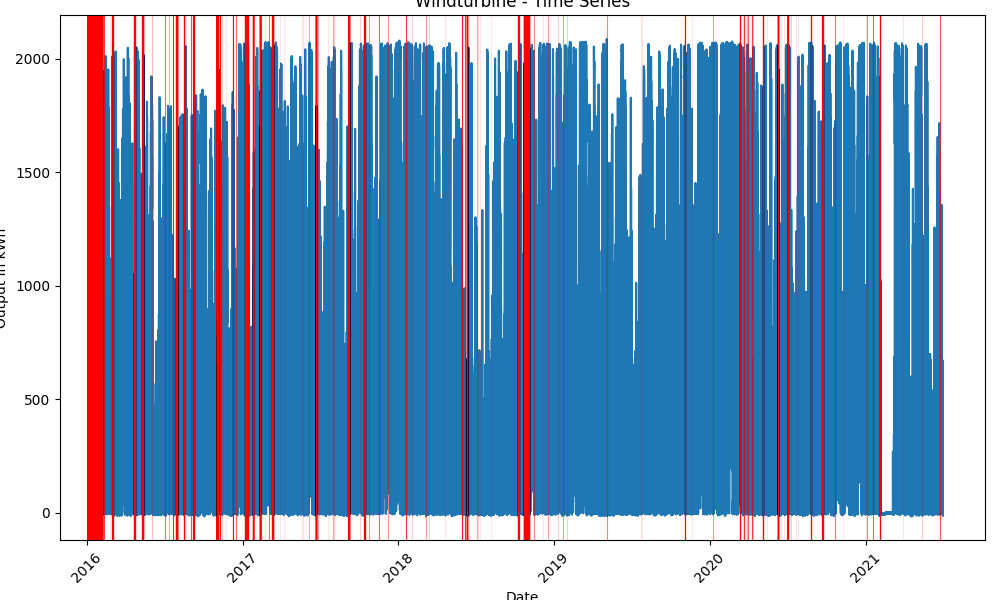
\includegraphics[width=\linewidth]{graphs/data/Windturbine - Time Series.png}
    \caption{Complete Power Output - Kelmarsh \#6}
    \label{fig:Kelmarsh-missing-values}
\end{figure}

This visualization reveals that the majority of missing data occurs at the beginning of the time series, suggesting that not all turbines were monitored from the start. As a result, all initial missing values, as well as sequences in each time series lasting more than three hours, are omitted from the analysis, as their retention offers no benefit to the forecasting task. These outages are likely due to maintenance activities. The issue of excessive outliers in three of the six turbines at Kelmarsh remains. Outliers have been defined as:
\begin{equation}
    |\text{outlier}| \geq 3 \times \left( \frac{x - \mu}{\sigma} \right)
\end{equation}
The threshold of three, rather than the more conventional two, accounts for extreme wind speeds particularly prevalent in coastal areas. To illustrate the potential outliers, all data points for the Kelmarsh wind park have been visualized using a kernel density estimation. The left part of figure \ref{fig:Kelmarsh-distribution} shows that the majority of values cluster around zero, indicating no electricity output, which could suggest inactive turbines due to operational decisions unrelated to wind conditions, such as economic considerations or grid capacity. To validate this, a detailed analysis of turbine 6 was conducted to determine the frequency with which it was turned away from the wind, defined as:
\begin{equation}
    \text{out of wind} = \text{Wind speed (m/s)} > 3 \land \text{Power (kW)} < 1 
\end{equation}
resulting in 8,705 instances, or 3.16\% of all data points being flagged. Consequently, these data points are removed as their inclusion is influenced more by market or grid demands rather than meteorological conditions. The extent can also be seen in the visualization of the $6^th$ turbine in the right figure \ref{fig:Kelmarsh-distribution}

\begin{figure}[h!]
    \centering
    \begin{subfigure}[b]{0.45\linewidth}
        \centering
        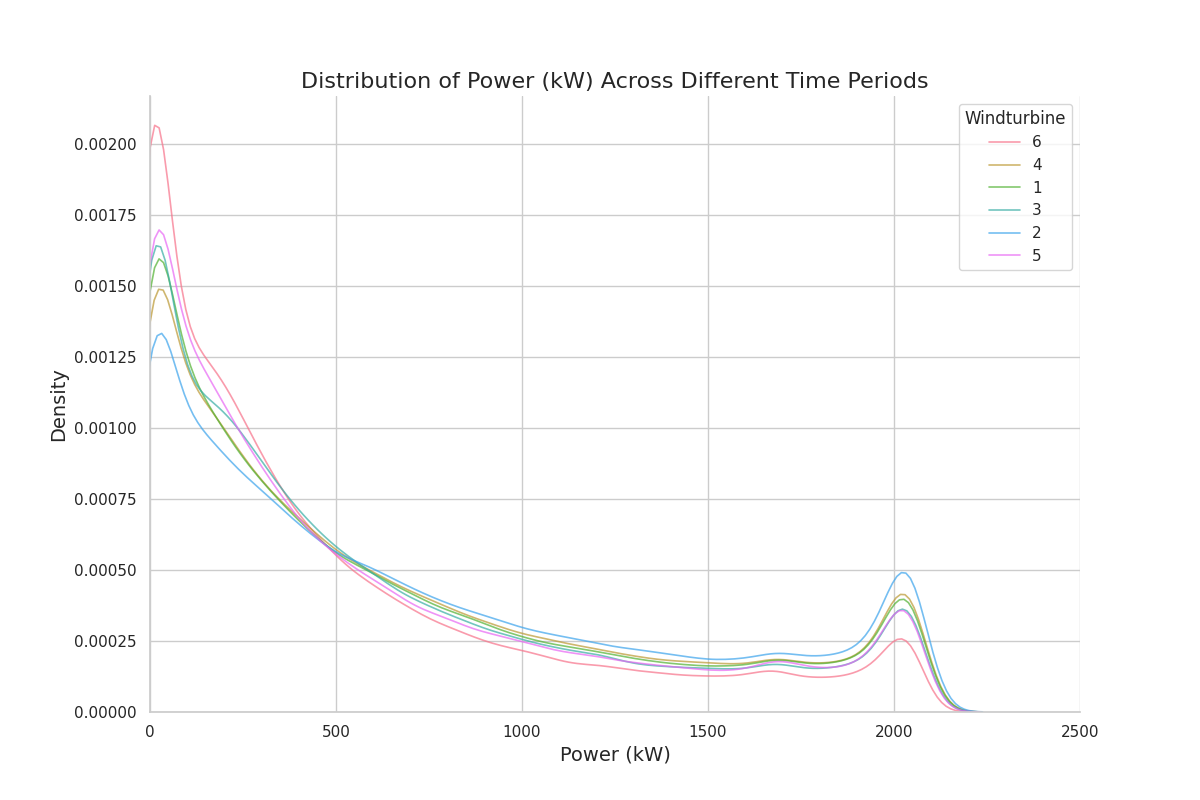
\includegraphics[width=\linewidth]{graphs/data/Kelmarsh_output_distribution.png}
        \caption{total}
    \end{subfigure}
    \begin{subfigure}[b]{0.45\linewidth}
        \centering
        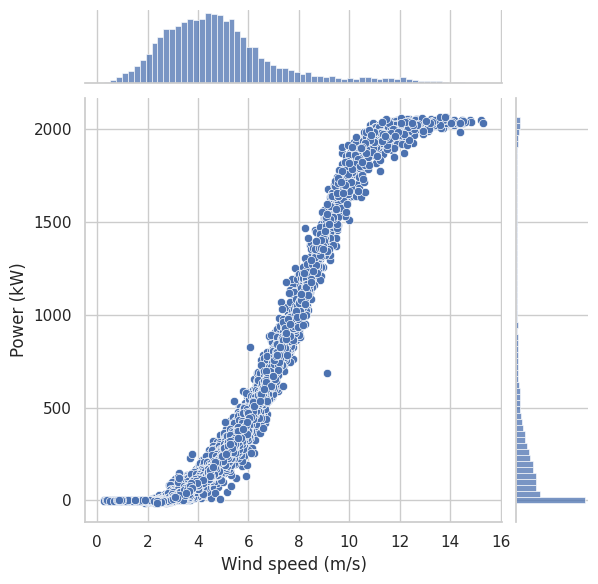
\includegraphics[width=\linewidth]{graphs/data/Corr_Wind_Power.png}
        \caption{\#6}
    \end{subfigure}
    \caption{Kelmarsh power distribution}
    \label{fig:Kelmarsh-distribution}
\end{figure}

\section{Methodology}

This study evaluates several forecasting models including multiple transformer architectures, and a benchmark model. The benchmark chosen is the linear regression model, picked for its usage in time series forecasting across various studies and the low complexity and thus resource efficient training as \cite{linear_forecasting_survey} shows in their literature review. The deep learning models employed are sourced from established GitHub repositories. The selection of transformer models includes both models from literature and a custom-built shallow transformer to explore the impact of network depth on forecasting accuracy. Forecasting horizons are set at 10 minutes, 1 hour, 6 hours, and 24 hours, aligning the longest with typical forecasts for spot market auctions to present a real world application as \cite{spot_market_forecasting} have shown in their work.

Evaluating the trade-off between increased predictive accuracy and the computational cost incurred is complex. In scalable environments, even marginal accuracy improvements can justify significant development expenditures. Initially, the data undergoes preprocessing to identify outliers and missing values, which could potentially influence model performance. Subsequently, it is processed through the various models, with performance compared across established metrics. Results are systematically tabulated and graphically presented to facilitate clear comparisons.

A critical consideration remains: determining the most meaningful way to assess model effectiveness. Beyond accuracy, factors such as training time, resource consumption, and the ease of interpretation for a broader audience are also crucial. The newly developed model aims for robust generalization across datasets, intentionally omitting specialized layers for seasonal decomposition or trend analysis found in other models.


\subsection{Model Evaluation}
\subsubsection{Error Metrics}

Evaluating the success of a model necessitates standardized methods to compare its performance accurately. In regression analysis, the effectiveness of a model is commonly assessed by the magnitude of its error; the smaller the error, the better the model's performance. Among the standard metrics used are:

Mean Absolute Error (MAE) is a straightforward metric for assessing regression model performance. It is calculated as the average of the absolute differences between predicted and actual values. The formula for MAE is given by:

\begin{equation}\label{eq:MAE}
\text{MAE} = \frac{1}{n} \sum_{i=1}^{n} \left| y_i - \hat{y}_i \right|
\end{equation}


where $y_i$ and $\hat{y}_i$ represent the actual and predicted values, respectively, and $n$ is the total number of observations. MAE offers an easily interpretable metric, applying a linear penalty for each unit of error between the predicted and actual values which is expertly explained by \cite{MAE_RMSE}.

Mean Squared Error (MSE), another widely utilized metric, averages the squares of the prediction errors:

\begin{equation}\label{eq:MSE}
\text{MSE} = \frac{1}{n} \sum_{i=1}^{n} (y_i - \hat{y}_i)^2
\end{equation}

MSE is particularly sensitive to larger errors, thereby heavily penalizing larger deviations from actual values as shown by \cite{MSE}.

For probabilistic forecasts, traditional metrics like MAE and MSE may not suffice. The Continuous Ranked Probability Score (CRPS) is designed to handle probabilistic forecasts. It measures the accuracy of a probabilistic forecast and reduces to the MAE in the case of deterministic forecasts. CRPS is thus a versatile metric that can be used to evaluate both deterministic and probabilistic models. Moreover, it can also serve as a loss function in training models, replacing the conventional cross-entropy loss. This metric has been widely adopted for probabilistic weather forecasting, as evidenced in various studies \cite{CRPS_example_1, CRPS_example_2, CRPS_example_3}:

\begin{equation}\label{eq:CRPS}
    CRPS(F, x) = \int_{-\infty}^{\infty} ( F(y) - \mathcal{H}(y-x) )^{2} dy
\end{equation}

Here, $F$ represents the cumulative distribution function of the forecast variable $X$, and $x$ is the observed value. $F(y) = \mathbf{P}[X \leq y]$ denotes the probability that $X$ is less than or equal to $y$, and $\mathcal{H}$ is the Heaviside step function defined as:

\begin{equation}
    \mathcal{H} = \begin{cases}
        1, & \mathbb{R} \geq 0 \\
        0, & \text{otherwise}
    \end{cases}
\end{equation}

\subsubsection{Resource Efficiency}

Utilizing these error metrics allows for the exploration of a range of potential issues and areas of interest, such as the penalization of outliers. However, often overlooked are additional model evaluation metrics beyond accuracy, including resource efficiency and computational requirements as \cite{transformers-effectiveness} mentioned in their work. These aspects of encompassing the time to train and the intuitive interpretation of results are emphasized in this thesis, particularly the aspect of resource efficiency, as highlighted by \cite{AI_energy_consumption} and \cite{resource_awareness}. The growing size and complexity of machine learning models, along with the increasing volume of data needed for training, demand substantial computational resources. This expansion has outstripped advancements in computing hardware, storage infrastructure, and networking capabilities, leading to sustainability challenges. While some initiatives, like those discussed in \cite{Informer}, have aimed to enhance computational efficiency, their focus has primarily been on reducing training time rather than on overall resource efficiency.

Evaluating resource efficiency presents challenges due to the absence of a standardized framework and measurements. Although it is beyond the scope of this thesis to develop such frameworks, this research undertakes to map the resources utilized across different models when trained on identical data sets. Additionally, the time invested throughout the development process—including training, testing, and inference on cloud computing platforms—is meticulously recorded, evaluated, and scrutinized for potential improvements and savings. To achieve this, a monitoring function operates during the training, testing, and evaluation phases to track CPU, RAM, and GPU usage, as well as the duration of model training. These metrics are recorded every second; although this monitoring consumes some resources itself, it is uniformly applied across all models, thereby normalizing the impact of its resource consumption. Ultimately, the focus is on analyzing average and peak usage metrics to determine which models are most cost-effective in terms of computational power utilization.


\subsection{Linear Models}

The linear model employed in this thesis serves as a benchmark against the more complex models. This benchmarking approach assumes that the more sophisticated models should outperform the simpler linear model. If the complex models do not exceed or at least match the performance of the linear model, they are considered inadequate for the tasks at hand and are subsequently disregarded.

The linear model is configured under the same initial conditions as the other models; it uses the same lags, operates in a multivariate context, and accesses identical datasets for training, validation, and testing phases. It does not incorporate components for seasonal decomposition or trend analysis, focusing instead on achieving robust performance without these elements to enhance its generalizability. This approach aligns with the Single-Layer-Perceptron setup used in the study by \cite{transformers-effectiveness}, picked for its utility in generating weights for the weighted mean CRPS loss function.

To maintain simplicity, the model consists of a single linear layer, mirroring the functionality of a traditional ordinary least squares regression. This simplicity is expected to facilitate the fastest training times and the lowest resource usage among the evaluated models. Additionally, since this model processes the same batches from the data loader as the other models, its training can be efficiently parallelized, further enhancing the speed of the training process.


\subsection{DeepLearning Models}

The objective of this section is to develop a tailored Transformer model for time series forecasting. This is achieved not by designing a model from scratch but by analyzing various published models to discern what unique contributions each model offers to this field. A critical evaluation is undertaken to understand how the model diverges from the traditional Transformer architecture and to assess whether these modifications yield benefits for the specific datasets used in this study.

As deep learning models are central to this research, an extensive evaluation of their performance is conducted. With each model introducing a different approach to the same forecasting challenge, a detailed comparison of all Transformer models is essential. This comparison aims to determine which architectures and strategies deliver superior performance.


\subsubsection{Vanilla Transformer}

The vanilla Transformer serves as a baseline model, closely mirroring the original architecture introduced by \cite{vanilla-transformer}, which employs the attention mechanism without specific optimizations for time series forecasting. This model does not include additional layers for seasonal decomposition or other time series-specific enhancements. It retains the standard encoder-decoder structure with fully connected layers and is expected to consume significant resources due to its unmodified complexity.

The implementation of this model is sourced from a GitHub repository \footnote{\url{https://github.com/thuml/Autoformer/blob/main/models/Transformer.py}}, ensuring compatibility with the tensor sizes used in other models like the Informer. For this thesis, while the fundamental transformer-specific components are adopted from the repository, modifications have been made to the framework around this model to align it with the other models.

\begin{figure}
    \centering
    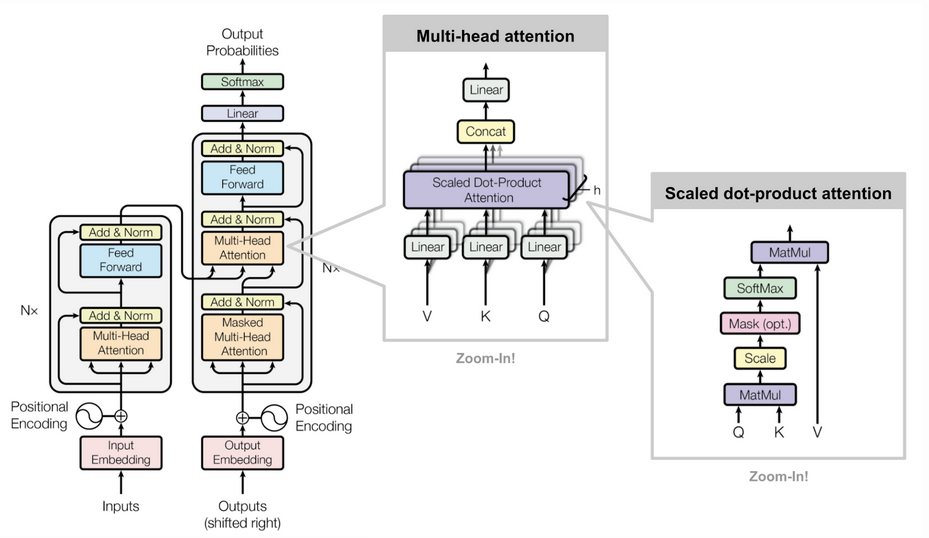
\includegraphics[width=\linewidth]{graphs/models/VanillaTransformer.png}
    \caption{Vanilla Transformer Architecture}
    \label{fig:VanillaTransformer_architecture}
\end{figure}

Detailed discussions on the functionalities of this Transformer model can be found in the work by \cite{vanilla-transformer}. However, alterations have been made for this thesis, particularly in the embedding techniques. The embedding function from the eFormer model, which utilizes the time2vec method as described by \cite{time2vec}, replaces the complex original embedding framework. Changes were also made to the output layer to streamline the model, these adjustment not only standardize function use across models but also enhance code generalization and maintainability in this thesis.


\subsubsection{Informer}

The Informer, developed by \cite{Informer}, distinguishes itself as a model capable of multivariate probabilistic time series forecasting, which contrasts with the typical univariate approaches as practiced by \cite{transformer_univariate_forecasting}. One of its most significant innovations is the reduction of computational demands associated with the attention mechanism, thus lessening memory usage in the encoder and decoder layers. This is accomplished through an improvement in the self-attention calculation complexity, typically represented by
\begin{equation*}
    O(T^2 \cdot D)
\end{equation*}
where $T$ is the length of the time series and $D$ is the dimension of the hidden states. The quadratic dependence on $T$ can become problematic for long sequences. The authors address this by introducing the ProbSparse method, which reduces complexity to
\begin{equation*}
    O(T \cdot \log{T}) .
\end{equation*}
This method differentiates between 'active' and 'lazy' components of the computation, focusing on the more impactful 'active' parts and disregarding the 'lazy' ones that contribute minimally to the attention mechanism.

\begin{figure}
    \centering
    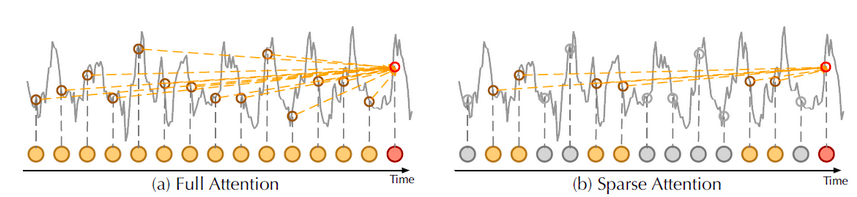
\includegraphics[width=\linewidth]{graphs/models/Sparse_Attention_Example.png}
    \caption{Informer: Sparse Attention}
    \label{fig:enter-label}
\end{figure}

Moreover, the Informer manages memory constraints effectively by implementing a Distilling operation, which condenses the input size between layers by halving it, thus significantly reducing memory requirements for handling longer sequences.

Another innovative feature of the Informer is the introduction of Probabilistic Time Embedding. This approach goes beyond simple vector encoding of data by accounting for uncertainties inherent in time-related information. Each time step's embedding is treated as a distribution rather than a fixed vector, allowing for multiple potential representations that capture the inherent uncertainty or variability at that moment. This probabilistic embedding is beneficial in scenarios where the time variable is crucial and its impact cannot be deterministically modeled. By accommodating a range of possible embeddings, the Informer can better handle uncertainties in system states or external factors not explicitly included in the model, enhancing the model’s robustness during both training and inference phases.


\subsection{eFormer}

The eFormer is positioned as the central point of this thesis, aiming to be a domain-specific probabilistic transformer model that surpasses more generalized models such as the Informer by \cite{Informer}. While forecast accuracy remains a primary performance metric, another critical aspect of evaluating the eFormer is its training time and resource consumption, reflecting its design goal to be as resource-efficient as possible. This efficiency is achieved by eliminating the decoder section and minimizing the number of layers and attention heads compared to similar models. Instead of developing new components, this model strategically integrates existing elements from prior research to find the optimal configuration for achieving its objectives.

The architectural framework of the eFormer incorporates time2vec embeddings as developed by \cite{time2vec}, combined with the positional encoding techniques from \cite{vanilla-transformer}. It also includes a sparse-attention mechanism that reduces computational complexity, as proposed by \cite{Informer}.The architecture is of deterministic nature and focuses solely on learning the mean values during training. This approach, while less resource-intensive, offers limited insights into the uncertainty of the forecasts, compared to probabilistic models. To enhance efficiency further, the model utilizes the early stopping technique to conserve resources and curtail training time if there is no significant change in loss, preventing redundant computational expenditure.


\subsubsection{Data Loader}

The data loader plays a crucial role in preparing the input datasets for the transformer models by ensuring proper dimensionality and preparing batches of the data. This setup allows parallel processing and represents the final phase of data engineering within the model pipeline. Initially, the dataset undergoes a transformation where it is shifted by $n$ timestamps—determined by the \textit{look\_back} hyperparameter to form a new data frame with the shape 
\begin{equation*}
    (\text{dependent variable}(look\_back + 1) + \text{independent variable}(look\_back), \text{time stamps})
\end{equation*}
Each row in this data frame represents an independent observation, where the first value is the ground truth and subsequent values are the lagged instances of both dependent and independent variables. The inclusion of future values of the dependent variable at the same timestamp as the true value is deliberately avoided to prevent the model from inadvertently learning from future data, therefor no masking is needed.

After the lag transformation, the data is partitioned into training, testing, and validation sets, incorporating shuffling to ensure that each split encompasses a diverse range of scenarios rather than contiguous segments, which might not fully capture long-term trends or seasonal effects in all three datasets, as only one set may hold a specific trend. An illustrative example of the importance of this method can be seen in the changed electricity consumption patterns during the COVID-19 pandemic, as discussed in \cite{COVID_electric_consumption}. To avoid such coincidences the data is shuffled before splitting, this does not effect the overall structure since every row is a full time series on its own.

To ensure compatibility with the model's batch processing requirements, the three datasets are further reshaped to align with the designated batch size. This adjustment occasionally necessitates the removal of the oldest $n$ entries that do not fit the batch size configuration, which, despite resulting in the loss of some data, is generally insignificant given the large scale of the 19 datasets, typically encompassing around 300,000 rows each. The processed data is then split into separate tensors for features and labels, which are subsequently loaded into the model using the \textit{torch.DataLoader} function. Within this framework, the training data is shuffled to introduce additional randomness, while the validation and testing sets remain sequential to preserve their temporal integrity.


\subsubsection{Embeddings \& Positional Encodings}

In the exploration of time series embeddings, \cite{time2vec} introduce a novel approach where time is treated as a periodic function using sine and cosine transformations. This method helps address the challenge of representing time cyclically, making it easier for models to interpret periodic patterns such as hours of the day. For the eFormer, these properties are utilized alongside positional encoding to enhance the model’s understanding of time sequence data.

To perform the time2vec transformation, the input tensor $\tau$ undergoes a sinusoidal transformation, followed by a linear transformation, with the results concatenated to form the final embeddings:
\begin{align}\label{eq:sin-transform}
    V_1 &= \sin(\tau \cdot W + B) \\
    V_2 &= \tau \cdot W_0 + B_0 \\
    t2v(\tau) &= V_1 \oplus V_2
\end{align}
The sine transformation \ref{eq:sin-transform} is based on the \textit{torch.sin} function, where the input tensor $\tau$ is multiplied with a weight matrix $W$ and the biases $B$ are added before the sin application. Both the weights and biases consist of randomly generated values from a standard normal distribution with $\mathcal{N}(0,1)$. This also can be performed using the cosine instead of the sine function. While the sinusoidal transformation captures the periodic time dependencies, the linear transformation exists to identify possible trends, and linear relationships in the underlying data. The variables used in the linear transformation serve as the input vector $\tau$, the weights $W_0$ and the biases $B_0$, with a difference in the dimensionality, since the weights and biases are only of dimension 1.

During the generation of embeddings, the raw data points loose their time stamps, which poses a challenge for transformer models that do not inherently account for sequence order due to their multi-head attention architecture. Positional encoding is introduced to circumvent this by providing temporal context that aids in maintaining the sequence's chronological order:
\begin{align}\label{eq:pos-encoding}
    PE(pos, 2i) &= sin \left( \frac{pos}{(2 \cdot time \; series \; length)^{2i / d_{model}}} \right) \\
    PE(pos, 2i + 1) &= cos \left( \frac{pos}{(2 \cdot time \; series \; length)^{2i / d_{model}}} \right)
\end{align}
This technique, introduced by \cite{vanilla-transformer}, employs sine and cosine functions to encode positional information based on the length of the entire time series, where $d_{model}$ is the dimensionality of the embeddings and $PE(pos, i)$ represents the final positional encoding at position $pos$ and dimension $i$, facilitating the model's interpretation of relative and absolute positioning of data points within the time series.

Finally, the embeddings and positional encodings are combined:
\begin{equation}
    Encoded(\tau) = t2v(\tau) + PE(pos, i)
\end{equation}
This method not only preserves the sequential order of the data but also allows the model to interpret and learn from the temporal data effectively.


\subsubsection{Sparse Attention}

In this implementation, the sparse attention mechanism serves as a substitute for the traditional vanilla attention mechanism, focusing on excluding segments of the time series deemed not significant for model predictions. This selective attention process is enabled by set thresholds established through the \textit{attention\_dropout} and \textit{prob\_sparse\_factor} hyperparameters, enabling the model to efficiently manage the relevance of data points throughout the sequence.

\begin{figure}
    \centering
    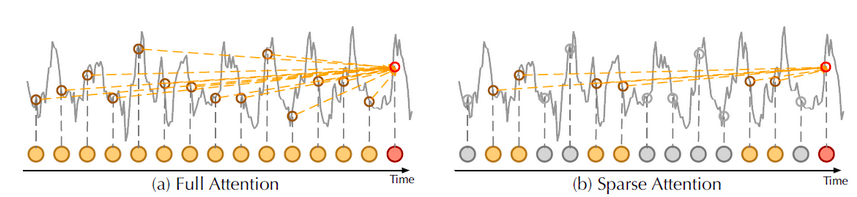
\includegraphics[width=\linewidth]{graphs/models/Sparse_Attention_Example.png}
    \caption{Comparison of Vanilla Self-Attention and Sparse Attention, picture taken from \cite{Informer}}
    \label{fig:sparse_attention}
\end{figure}

Unlike other transformer architectures, this model does not employ a masking strategy since there is no decoder to shield information from and each time series in a batch only consists of past values without the chance to access different time series'. Instead, an empty vector placeholder represents the future time horizons targeted for prediction. These future timestamps undergo the same positional encoding process as the embeddings, ensuring that the model's 'decoder' segment simply extends the prediction tasks to unseen future timestamps. This is achieved by utilising a recurrent forecasting method as described by \cite{recurrent_forecasting} where only one step is forecasted each iteration until the goal of a $n$-step forecast is reached.

The structure of the transformers using the sparse attention mechanism is depicted in Figure \ref{fig:eFormer_sparse}. This approach not only simplifies the architectural complexity but also optimizes computational efficiency by focusing processing power on data segments with the highest relevance, thereby maintaining or enhancing predictive accuracy while managing resource use effectively.

\begin{figure}
    \hspace*{\fill}
    \begin{subfigure}[b]{0.4\linewidth}
        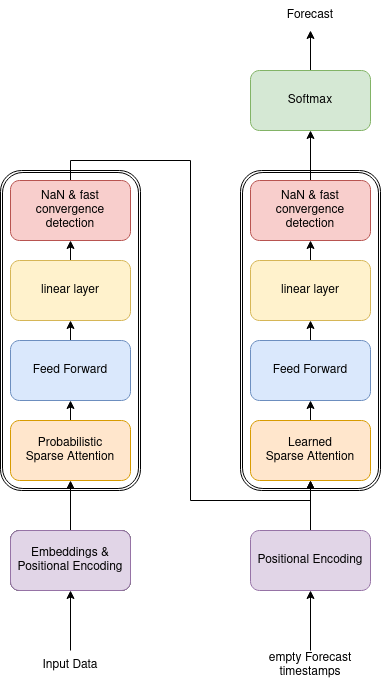
\includegraphics[width=\linewidth]{graphs/models/eFormer_probSparse.png}
        \caption{probabilistic}        
    \end{subfigure}
    \hfill
    \begin{subfigure}[b]{0.4\linewidth}
        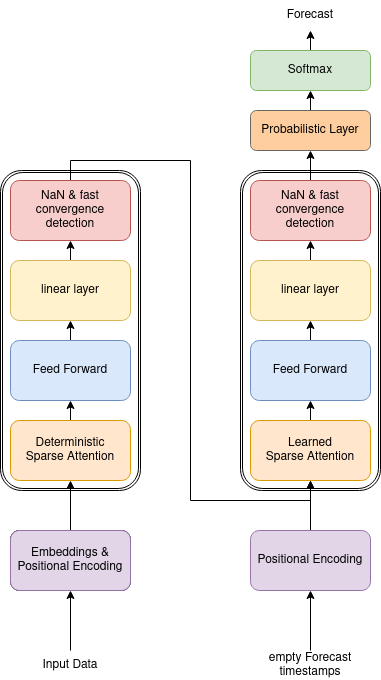
\includegraphics[width=\linewidth]{graphs/models/eFormer_det_sparse.png}
        \caption{deterministic}
    \end{subfigure}
    \hspace*{\fill}
    \caption{eFormer Sparse Attention}
    \label{fig:eFormer_sparse}
\end{figure}

Reducing the computational overhead is accomplished by building subsets of the key vectors $K$ by sampling for each query vector $Q$. These vectors have the dimensions $[B, H, L_K, D]$ and $[B, H, L_Q, E]$ respectively which is the same as in the Informer model by \cite{Informer}, where:
\begin{itemize}
    \item $B$ denotes the batch size,
    \item $H$ represents the number of multi-head attentions,
    \item $L_K$ and $L_Q$ are the lengths of the key and query sequences,
    \item $D$ and $E$ are the dimensions of the key and query vectors.
\end{itemize}

This is implemented in the \textit{ProbAttention} class, where the parameter $U_{part}$ describes the size of the sample and is determined by the equation:
\begin{equation}
    U_{part} = c \ceil*{\log(L_K)}
\end{equation}
Here, $c$ is a hyperparameter, $L_K$ is the length of the sampled key sequence, and $\ceil*{\cdot}$ is the ceiling function, ensuring that $U_{part}$ remains an integer. The logarithmic relationship helps maintain computational scalability by preventing the sampling complexity from increasing linearly with the input size.

Sampling from the key vector $K$ is executed using the \textit{torch.randint} function, producing a tensor $K_{sample}$ of length $U_{part}$. The dot-product between $Q$ and $K_{sample}^T$ is calculated:
\begin{equation}
    QK^T_{sample} = Q \cdot K_{sample}
\end{equation}

This dot-product calculation is the key aspect in the reduced computational load. The result $QK^T_{sample}$ then undergoes a sparsity measurement to evaluate the potential impact of each query on the output. This measure is computed as follows:
\begin{equation}
    M = \max(QK^T_{sample}) - \frac{\sum^K_{i=1} QK^T_{sample}}{L_K}
\end{equation}
From this measurement, the top $n$ values are selected based on their potential impact, where $n$ is derived similarly to $U_{part}$:
\begin{equation}
    n = c \ceil*{\log(L_Q)}
\end{equation}
with the same logarithmic scaling applied.

The final computation involves the dot-product of the selected queries with the entire key vector:
\begin{equation}
    Q_{selected}K^T = Q_{selected} \cdot K
\end{equation}

This selective computation significantly reduces the overall complexity to $O(T \log(T))$, aligning with the efficiency goals set forth by \cite{Informer}, and ensuring that the model remains scalable even as input lengths increase.


The computation of attention scores is an important step in the functioning of the sparse attention mechanism and is executed within the same class that handles the reduced dot-product calculations. Initially, context vectors are derived as the mean of the value tensor $V$ with dimensions $[B,H,L_V,D]$. This simplification is possible in this model as there is no need for masking future tokens due to the absence of a traditional decoder, therefor streamlining the computation further.

The following step involves updating the context vectors. This is achieved by first normalizing the attention scores calculated from the dot-product to enhance numerical stability before applying the softmax function. The scores are scaled down by the dimensionality of the heads to prevent excessively large exponents in the softmax function, which could lead to numerical instability:

\begin{align}
    a_{ijk} &= a_{ijk} \frac{1}{\sqrt{D}} \\
    a_{ijk} &= \frac{e^{a_{ijk}}}{\sum^{L_K}_{k=1}e^{a_{ijk}}}
\end{align}

Here, $a_{ijk}$ represents the normalized attention weight for the $k$-th key vector relative to the $j$-th query within the $i$-th batch and $D$ as the dimensionality of each head. The updated context vector is further processed for each selected query index by aggregating information across the value sequence, weighted by the relevance of each value vector as determined by the computed attention scores:
\begin{equation}
    context_{in}[:,:,index,:] = \sum^{L_K}_{k=1} a_{ijk} \cdot V_{:,:,k,:}
\end{equation}
The weights $a_{ijk}$ utilized in updating the context vectors are derived from the normalized attention scores, ensuring that each value's contribution is proportionate to its assessed relevance.

The Attention Layer combines all the previously discussed functions, ensuring the output tensor is correctly dimensioned. This layer is essential in the multi-head attention mechanism, enabling parallel computation to optimize processing efficiency. The implementation involves four steps, it starts with a linear transformations of the query, key, and value matrices to align them to the appropriate dimensions for subsequent computations:
\begin{align}
    Q' &= QW^Q \\
    K' &= KW^K \\
    V' &= VW^V
\end{align}
Here, $W^{Q, K, V}$ are the weight matrices derived from the linear layers, designed to prepare the inputs for parallel processing across the multiple attention heads.

Next the attention scores are calculated utilizing the methodologies detailed earlier:
\begin{equation}\label{eq:Encoder-Attention}
    Attention(Q', K', V') = \text{softmax} \left( \frac{Q'K'^T}{\sqrt{D / H}} \right) V'
\end{equation}
In this formula, $Q'K'^T$ represents the dot product forming the basis of the attention scores, while $\sqrt{D / H}$ is a scaling factor that helps maintain numerical stability by preventing excessively large values.

Following the computation of attention, the results from different heads are aggregated. This mixing is essential for the model to capture various aspects of the same data, providing a richer and more detailed representation. As shown in previous studies by \cite{multi-head-mixing, mulit-head-mixing2}, this approach not only enhances data representation but also promotes better generalization and faster convergence by allowing each head to specialize and subsequently synergize their findings.

The final step involves another linear projection to reshape the combined attention outputs from equation \ref{eq:Encoder-Attention} to the required dimensions, setting the stage for further processing or output generation.

The Sparse Attention Model's Encoder has been outlined previously, focusing on streamlining operations to enhance computational efficiency. The corresponding Decoder part, in keeping with the minimalist idea, contains positional encoding for forecasted values and using cross attention to bring together the results from the attention heads in the encoder.

This Decoder is a customized variant of the standard transformer decoder, specifically adapted for time series data and the sparse attention strategy employed in the encoder. It incorporates dropout to prevent overfitting and utilises the ReLu activation function. The inputs to this decoder are the encoder's output tensor and the generated positional encodings for the forecasted values. The forward pass of the decoder consists of several steps: positional encoding, cross-attention, a feed-forward network, layer normalization, and ultimately, output generation. While this sequence implies a complex process, it is streamlined by omitting elements like self-attention solely within the decoder and its associated masking. The only additional element aside from the core functions is the feed-forward network, which includes two convolutional layers.

The positional encoding, identical to that used in the encoder as detailed in equation \ref{eq:pos-encoding}, ensures continuity in the time representation. The cross-attention layer processes inputs from both the decoder and the encoder. Here, the decoder's positional encodings serve as queries $Q$, while the keys $K$ and values $V$ are derived from the encoder. This integration is articulated in the modified equation:
\begin{equation}\label{eq:Decoder-CrossAttention}
    Attention(Q_{Decoder}, K_{Encoder}, V_{Encoder}) = \text{softmax} \left( \frac{Q_{Decoder} K_{Encoder}^T}{\sqrt{D / H}} \right) V_{Encoder}
\end{equation}
In this setup, keys and values undergo sampling again, as previously described, thus reducing the volume of data processed and maintaining computational efficiency.

The feed-forward network within the decoder is crucial for capturing complex patterns in the observed data through its non-linear activation function. The network begins with a convolutional layer that performs an element-wise transformation, using a kernel of size 1. This transformation adjusts the dimensionality from the initial model dimension $d_{model}$ to that of the hidden layer of the feed-forward network $d_{ff}$:

\begin{align}
    FFN_1 &= \text{ReLU}(\text{Conv}_{\text{kernelsize} = 1}(\text{Attention}(Q_{Decoder}, K_{Encoder}, V_{Encoder}))), \\
    FFN_2 &= \text{Conv}_{\text{kernelsize} = 1}(FFN_1)
\end{align}

\begin{align}\label{eq: decoder-ffn}
    FFN_1 &= ReLu(Conv_{kernelsize = 1}(Attention(Q_{Decoder}, K_{Encoder}, V_{Encoder}))) \\
    FFN_2 &= Conv_{kernelsize = 1}(FFN_1)
\end{align}

To ensure compatibility with subsequent layers, the output from $FFN_1$ is transformed back to $d_{model}$ dimensions using a second convolutional layer, which lacks an activation function as the activation has already been applied in the first layer. The adoption of convolutional layers, rather than fully connected dense layers, offers several advantages including parameter sharing, parallelization, and application of filters on smaller regions due to the small kernel size which provides benefits to capturing short term dependencies.

The next phase incorporates layer normalization to enhance the model's stability and address potential issues with vanishing gradients. This normalization is applied to both the outputs from the attention mechanism and the feed-forward network:
\begin{align}
    \text{Attention}(Q,K,V) &= \text{LayerNorm}(\text{Attention}(Q,K,V) + \text{Dropout}(\text{Attention}(Q,K,V))), \\
    FFN_3 &= \text{LayerNorm}(\text{Attention}(Q,K,V) + \text{Dropout}(FFN_2))
\end{align}
Here, dropout is set at $0.1$, effectively deactivating a fraction of the neurons to promote model generalization by compelling the network to explore alternative pathways during training.

In the final step, the processed tensor from $FFN_3$ is transformed into the forecasted values via a linear projection:
\begin{equation}
    \text{forecast} = FFN_3 W + b
\end{equation}
where $W$ and $b$ represent the weights and biases of the linear layer, respectively. After this transformation the forecast is an interpretable value which can be compared to the ground truth, thus the error can be calculated and the back propagation steps can start to update the weights.


\subsubsection{Loss Function}

As outlined earlier in the description of the eFormer, a custom loss function is adopted to enhance the model's performance with both probabilistic and deterministic data. The chosen metric is the Continuous Ranked Probability Score (CRPS), which effectively extends the Mean Absolute Error (MAE) to accommodate the specific case of probabilistic forecasts. For deterministic models, CRPS simplifies to calculating the MAE, allowing for a unified approach to evaluating both types of models.

In the implemented version, the CRPS is further customized to integrate weighting mechanisms that prioritize certain predictions over others, a modification from the standard CRPS where each prediction contributes equally to the overall loss:
\begin{equation}
    CRPS = \frac{1}{N} \sum^N_{i = 1} w_i (CDF_{forecast_i} - \mathcal{I}(f_i, t))^2
\end{equation}
where $w_i$ represents weights derived from the decoder, enhancing the impact of specific predictions on the loss calculation based on their respective significance.

The calculation of CRPS involves several steps. Initially, all input dimensions are standardized to ensure uniformity. This includes removing singleton dimensions from the predictions and computing the mean across the last dimension of the weights to align all input vectors to the sequence length defined in the hyperparameters. The CRPS employs a cumulative distribution function (CDF), necessitating the sorting of forecast values before their cumulative sums can be computed:
\begin{equation}
    CDF = \frac{1}{N} \sum^N_{i = 1} \mathcal{I}(f_i < f)
\end{equation}
with $f_i$ as the forecasted values, $N$ as the total number of forecasts, and $\mathcal{I}$ as an indicator function approximated by the cumulative sum over the forecasts. The indicator function $\mathcal{I}$ is defined as:
\begin{equation}
    \mathcal{I}(f, t) = \begin{cases}
        1, & f > t \\
        0, & \text{otherwise}
    \end{cases}
\end{equation}
This function assesses whether each forecasted value exceeds the true value, integrating these comparisons into the CRPS computation.

Additionally, standard loss functions like MSE and L1 Loss are also utilized, drawing from their existing use in the literature, as noted in studies like the Informer paper. These functions are implemented using the \textit{torch.nn} package, referencing the MSE and MAE error metrics previously introduced in equations \ref{eq:MSE} and \ref{eq:MAE}. These widespread metrics provide a reliable performance assessment alongside the more specialized CRPS.


\subsection{Experiment Setup}

The experimental setup and corresponding code for this thesis can be accessed via the \href{https://github.com/janbesler/Masterarbeit}{GitHub repository}. The experiments involve training the same models under varying parameters to assess their performance across different forecast horizons. A key variable in these experiments is the size of the look back window, which is adjusted according to the forecast horizon to capture a sufficient context from the data, as outlined in table \ref{tab:forecast-lookback}.

\begin{table}[h!]
  \begin{center}
    \caption{Combination of Forecast Horizon with Look Back Window Size}
    \begin{tabular}{c|c|c|c}
      \toprule
       & \multicolumn{3}{c}{\textbf{Look Back Window}} \\
      \textbf{Forecast Horizon} & 12 h & 48 h & 96 h \\
      \midrule
      10 min & x & & \\
      1 h & x & & \\
      12 h & & x & \\
      24 h & & & x \\
      \bottomrule
    \end{tabular}
    \label{tab:forecast-lookback}
  \end{center}
\end{table}

The embedding lengths for the experiments are set to $[32, 64, 128]$, chosen because they are powers of two, a common practice in computational settings as discussed by \cite{optimal_embedding_length}. Longer embedding lengths typically reduce the number of close matches between data points, as they provide a more detailed representation of the data, an effect described by \cite{introduction_embeddings}. However, excessively detailed embeddings can hinder the model's ability to generalize, as they may create too much distance between the data points in the embedding space.

Alongside varying embedding lengths, multiple loss functions are explored to ascertain any significant impact on performance. The loss functions implemented include custom CRPS, MSE, and L1 Loss, with these choices inspired by their prevalent use in existing studies such as those detailed in \cite{Informer, autoformer, cross-entropy_time-series}. The CRPS is particularly suited to probabilistic models, while MSE and L1 provide reliable benchmarks for performance comparison.

The models utilized in the experiments are:
\begin{multicols}{2}
\begin{itemize}
    \item Custom eFormer
    \item Vanilla Transformer
    \item Informer
    \item Single Layer Perceptron
\end{itemize}
\end{multicols}

Among these, the Single Layer Perceptron serves as a baseline benchmark, while the Vanilla Transformer, typically optimized for NLP tasks as \cite{vanilla-transformer} mentioned in their paper, provides a general deep learning benchmark. The eFormer and Informer are expected to excel in terms of accuracy and computational efficiency due to their specialized attention mechanisms designed specifically for time series data. The simplest and most cost-effective model, the Single Layer Perceptron, is anticipated to be the least resource-intensive due to its minimalistic design.


\section{Results}

The results from each experiment are meticulously organized into distinct data frames, which are then aggregated into a dictionary to facilitate easy access based on the defined keys. These data frames are categorized into three primary groups:
\begin{multicols}{2}
\begin{itemize}
    \item Hardware Usage
    \item Epoch Duration \& Loss
    \item Predictions \& Labels
\end{itemize}
\end{multicols}

The hardware usage metrics are recorded every second across CPU, RAM, and GPU, providing a measure of the maximum and average resource demand during the training and validation phase. This frequent measurement interval was chosen to capture transient spikes in resource usage, initially noted to exceed one second in duration during test runs. However, intervals less frequent than one second were avoided to prevent excessive system burden and to maintain manageable data set sizes. The hardware configurations include a V100 NVIDIA server with 51GB of RAM and 16GB of GPU RAM, except for the Vanilla Transformer with a forecast length of 144, where an A100 NVIDIA server with 80GB of RAM and 40GB of GPU RAM was utilized due to GPU limitations encountered with the V100.

The Epoch Duration \& Loss data frames capture the time taken for each training and validation cycle and the associated validation loss. These measurements are important in evaluating the models’ efficiency and effectiveness. The duration data is used in estimating computational cost efficiencies, critical for cloud computing environments like AWS or Lambda, where pricing models are time-based. The test loss on the other hand provides insights into each model's predictive accuracy. Rapid convergence is particularly favorable as it suggests that the models are not only achieving desirable accuracy but are also optimizing resource usage by minimizing necessary training time, this is approximated by the number of epochs during the training process.

The third group, encompassing Predictions \& Labels, primarily serves for visual analysis, with the assessment of the time series differences between the predicted and true values as a direct comparison and a comparison of their respective distributions.

The Test Loss stayed the same for the eFormer Model, and the deep learning models, the Loss function CRPS is therefor emitted from further experiments to save resources as it is not working as planned. This is shown in table \ref{tab:CRPS_convergence} where the convergence of the validation loss is shown across different models. Where the experiments have already been conducted, the information on the CRPS remains, but is it emitted in most results tables.

\begin{table}
    \footnotesize
    \centering
    \caption{CRPS Convergence}
    \begin{tabular}{l|S|S|S}
        \toprule
        \textbf{Epoch} & \textbf{eFormer} & \textbf{Vanilla Transformer} & \textbf{Informer} \\
        \midrule
        1 & 0.249272 & 0.249270 & 0.249290 \\
        2 & 0.249268 & 0.249268 & 0.249269 \\
        3 & 0.249268 & 0.249268 & 0.249268 \\
        4 & 0.249268 & 0.249268 & 0.249268 \\
        5 & 0.249268 & 0.249268 & 0.249268 \\
        6 & 0.249268 & 0.249268 & 0.249268 \\
        7 & 0.249268 & 0.249268 & 0.249268 \\
        8 & 0.249268 & 0.249268 & 0.249268 \\
        9 & 0.249268 &  & 0.249268 \\
        10 & 0.249268 &  & 0.249268 \\
        \bottomrule
    \end{tabular}
    \label{tab:CRPS_convergence}
\end{table}

Another setback are the missing values for the Informer model for the forecast horizons of $72$ and $144$, since the calculations took so long that the system aborted several times after 36 hours of running. 

\subsection{Hardware Usage}

In determining the appropriate hardware for training, it is essential to consider the maximum resource usage observed during the training processes. This maximum usage is a critical factor in selecting hardware specifications. Additionally, average usage metrics are crucial for estimating the power consumption of the servers employed. The observed spikes in RAM usage, detailed in the tables \ref{tab:vanillatransformer_hardware_f6}, \ref{tab:informer_hardware_f6}, and \ref{tab:eformer_hardware_f6}, are attributed to the substantial memory demands of handling over 5.5 million data points converted into time series. These initial spikes do not occur again with the same intensity after the data loader phase, suggesting that servers should be equipped with at least three times the average RAM capacity to efficiently manage peak loads during data loading. Regarding GPU usage, the average and maximum metrics are similar, indicating that there is no need for a buffer in GPU capacity for most of the training processes. With the batch size set at 512, the V100 servers employed are not fully utilized, opening the possibility to increase the training speed without additional GPU capacity.

CPU usage varies across models, but only in three instances, noted in tables \ref{tab:vanillatransformer_hardware_f6} and \ref{tab:vanillatransformer_hardware_emb64}, does the CPU reach its capacity limits, suggesting that CPU capacity is generally adequate for the tasks assigned.

An interesting observation is the increase in RAM usage with longer forecasting horizons across all models except the Informer, where RAM usage remains stable. This stability could indicate a more efficient data processing approach within the Informer model. For GPU usage, there is an expected increase with longer forecasting horizons due to larger matrices, although the difference between 1-step to 6-step forecasting is negligible. Specifically, the Vanilla Transformer shows a significant increase in GPU usage for longer horizons, whereas the eFormer model maintains consistent GPU usage across different loss functions, with only a moderate increase observed under the MSE Loss function for increasing forecast horizons until it reaches the similar values to the L1 Loss.

Overall, the MSE Loss function appears to require less or at most equal GPU resources compared to the L1 Loss function across all models and hyperparameters, while CPU and RAM usages remain comparable. This suggests that MSE Loss is generally less GPU-intensive, offering a potentially more resource-efficient option for model training.

\begin{table}
    \footnotesize
    \centering
    \caption{Linear Model Hardware Results}
    \begin{tabular}{l|l|S|S|S|S|S|S}
        \toprule
        \textbf{Loss} & \textbf{Forecast} & \multicolumn{3}{c|}{\textbf{max Usage}} & \multicolumn{3}{c}{\textbf{avg Usage}} \\
        \textbf{Function} & \textbf{Horizon} & \text{CPU (\%)} & \text{RAM (GB)} & \text{GPU (GB)} & \text{CPU (\%)} & \text{RAM (GB)} & \text{GPU (GB)} \\
        \midrule
        CRPS & 1 & 24.5 & 8.2529 & 0.416 & 15.5598 & 8.1493 & 0.416 \\
        MSE & 1 & 25.0 & 8.0487 & 0.3965 & 15.8084 & 7.8799 & 0.3936 \\
        L1 & 1 & 25.2 & 8.2727 & 0.416 & 15.8348 & 8.1863 & 0.416 \\
        \midrule
        CRPS & 6 & 24.2 & 8.2508 & 0.416 & 15.5146 & 8.1714 & 0.416 \\
        MSE & 6 & 25.6 & 8.1368 & 0.3965 & 15.8478 & 8.0447 & 0.3965 \\
        L1 & 6 & 25.5 & 8.3929 & 0.416 & 15.8739 & 8.2895 & 0.416 \\
        \midrule
        CRPS & 72 & 24.7 & 25.8702 & 0.416 & 15.5017 & 25.3396 & 0.416 \\
        MSE & 72 & 25.4 & 25.7994 & 0.3965 & 15.9529 & 25.051 & 0.3965 \\
        L1 & 72 & 23.8 & 25.9554 & 0.416 & 15.8362 & 24.9946 & 0.416 \\
        \midrule
        CRPS & 144 & 24.0 & 47.3446 & 0.416 & 15.4113 & 44.94 & 0.416 \\
        MSE & 144 & 25.6 & 47.4935 & 0.416 & 15.8783 & 45.869 & 0.416 \\
        L1 & 144 & 25.3 & 47.5861 & 0.416 & 15.8157 & 44.9186 & 0.416 \\
    \bottomrule
    \end{tabular}
    \label{tab:linear_hardware}
\end{table}

\begin{table}
    \footnotesize
    \centering
    \caption{eFormer Model Hardware Results for Forecast = 6}
    \begin{tabular}{l|l|S|S|S|S|S|S}
        \toprule
        \textbf{Loss} & \textbf{Embedding} & \multicolumn{3}{c|}{\textbf{max Usage}} & \multicolumn{3}{c}{\textbf{avg Usage}} \\
        \textbf{Function} & \textbf{Length} & \text{CPU (\%)} & \text{RAM (GB)} & \text{GPU (GB)} & \text{CPU (\%)} & \text{RAM (GB)} & \text{GPU (GB)} \\
        \midrule
        CRPS & 32 & 71.0 & 14.0473 & 1.5371 & 64.3825 & 13.9536 & 1.5371 \\
        MSE & 32 & 71.0 & 14.2312 & 0.873 & 64.0783 & 13.8792 & 0.8728 \\
        L1 & 32 & 71.8 & 14.0313 & 1.5352 & 65.0532 & 13.9467 & 1.5352 \\
        \midrule
        CRPS & 64 & 70.0 & 14.1169 & 1.5371 & 63.6695 & 14.047 & 1.5371 \\
        MSE & 64 & 71.1 & 14.0182 & 1.0938 & 63.7473 & 13.9465 & 1.0922 \\
        L1 & 64 & 71.2 & 14.041 & 1.5352 & 64.0915 & 13.9614 & 1.5352 \\
        \midrule
        CRPS & 128 & 66.5 & 14.1367 & 1.5371 & 60.1154 & 14.0306 & 1.5371 \\
        MSE & 128 & 66.6 & 14.0188 & 1.5352 & 60.964 & 13.9608 & 1.5333 \\
        L1 & 128 & 67.2 & 14.0407 & 1.5352 & 60.6614 & 13.9786 & 1.5352 \\
    \bottomrule
    \end{tabular}
    \label{tab:eformer_hardware_f6}
\end{table}

\begin{table}
    \footnotesize
    \centering
    \caption{Vanilla Transformer Model Hardware Results for Forecast = 6}
    \begin{tabular}{l|l|S|S|S|S|S|S}
        \toprule
        \textbf{Loss} & \textbf{Embedding} & \multicolumn{3}{c|}{\textbf{max Usage}} & \multicolumn{3}{c}{\textbf{avg Usage}} \\
        \textbf{Function} & \textbf{Length} & \text{CPU (\%)} & \text{RAM (GB)} & \text{GPU (GB)} & \text{CPU (\%)} & \text{RAM (GB)} & \text{GPU (GB)} \\
        \midrule
        MSE & 32 & 59.6 & 7.9908 & 1.0762 & 40.1941 & 7.9169 & 1.0711 \\
        L1 & 32 & 55.0 & 8.3419 & 1.6875 & 39.8451 & 8.2588 & 1.6875 \\
        \midrule
        MSE & 64 & 100.0 & 42.0759 & 2.9727 & 45.527 & 13.851 & 2.9648 \\
        L1 & 64 & 100.0 & 30.9259 & 2.9727 & 47.1468 & 13.4471 & 2.9727 \\
        \midrule
        MSE & 128 & 61.2 & 8.4467 & 1.6875 & 41.1515 & 8.3857 & 1.6747 \\
        L1 & 128 & 58.2 & 8.3387 & 1.6875 & 40.7646 & 8.2766 & 1.6875 \\
    \bottomrule
    \end{tabular}
    \label{tab:vanillatransformer_hardware_f6}
\end{table}

\begin{table}
    \footnotesize
    \centering
    \caption{Informer Model Hardware Results for Forecast = 6}
    \begin{tabular}{l|l|S|S|S|S|S|S}
        \toprule
        \textbf{Loss} & \textbf{Embedding} & \multicolumn{3}{c|}{\textbf{max Usage}} & \multicolumn{3}{c}{\textbf{avg Usage}} \\
        \textbf{Function} & \textbf{Length} & \text{CPU (\%)} & \text{RAM (GB)} & \text{GPU (GB)} & \text{CPU (\%)} & \text{RAM (GB)} & \text{GPU (GB)} \\
        \midrule
        MSE & 32 & 53.3 & 8.0623 & 0.7715 & 39.009 & 7.7727 & 0.7686 \\
        L1 & 32 & 53.7 & 8.4872 & 1.4902 & 38.9235 & 8.3968 & 1.4902 \\
        \midrule
        MSE & 64 & 52.2 & 8.3992 & 1.0234 & 37.7099 & 8.3183 & 1.0225 \\
        L1 & 64 & 51.0 & 8.5536 & 1.4902 & 38.4718 & 8.4442 & 1.4902 \\
        \midrule
        MSE & 128 & 54.2 & 8.4896 & 1.4902 & 38.0454 & 8.3917 & 1.4878 \\
        L1 & 128 & 50.7 & 8.5385 & 1.4902 & 37.573 & 8.4417 & 1.4902 \\
    \bottomrule
    \end{tabular}
    \label{tab:informer_hardware_f6}
\end{table}

\begin{table}
    \footnotesize
    \centering
    \caption{eFormer Model Hardware Results for Embedding Length = 32}
    \begin{tabular}{l|l|S|S|S|S|S|S}
        \toprule
        \textbf{Loss} & \textbf{Forecast} & \multicolumn{3}{c|}{\textbf{max Usage}} & \multicolumn{3}{c}{\textbf{avg Usage}} \\
        \textbf{Function} & \textbf{Horizon} & \text{CPU (\%)} & \text{RAM (GB)} & \text{GPU (GB)} & \text{CPU (\%)} & \text{RAM (GB)} & \text{GPU (GB)} \\
        \midrule
        MSE & 1 & 74.8 & 8.1822 & 0.8301 & 64.4926 & 8.0418 & 0.8121 \\
        L1 & 1 & 73.0 & 8.4206 & 3.3789 & 63.4702 & 8.3481 & 3.3789 \\
        \midrule
        MSE & 6 & 71.0 & 14.2312 & 0.873 & 64.0783 & 13.8792 & 0.8728 \\
        L1 & 6 & 73.6 & 8.4276 & 3.3789 & 63.9189 & 8.3514 & 3.3789 \\
        \midrule
        MSE & 72 & 65.6 & 26.3948 & 2.1035 & 54.1944 & 26.0339 & 2.0652 \\
        L1 & 72 & 62.5 & 26.2108 & 3.3789 & 52.6659 & 25.9123 & 3.3789 \\
        \midrule
        MSE & 144 & 56.1 & 47.7485 & 3.3789 & 45.1301 & 47.1554 & 3.3448 \\
        L1 & 144 & 55.9 & 47.9712 & 3.3789 & 45.5213 & 46.6185 & 3.3789 \\
    \bottomrule
    \end{tabular}
    \label{tab:eformer_hardware_emb32}
\end{table}

\begin{table}
    \footnotesize
    \centering
    \caption{Vanilla Transformer Model Hardware Results for Embedding Length = 64}
    \begin{tabular}{l|l|S|S|S|S|S|S}
        \toprule
        \textbf{Loss} & \textbf{Forecast} & \multicolumn{3}{c|}{\textbf{max Usage}} & \multicolumn{3}{c}{\textbf{avg Usage}} \\
        \textbf{Function} & \textbf{Horizon} & \text{CPU (\%)} & \text{RAM (GB)} & \text{GPU (GB)} & \text{CPU (\%)} & \text{RAM (GB)} & \text{GPU (GB)} \\
        \midrule
            MSE & 1 & 55.3 & 7.984 & 1.2461 & 40.5018 & 7.8214 & 1.2361 \\
        L1 & 1 & 55.9 & 7.9927 & 1.2266 & 41.3934 & 7.6841 & 1.2159 \\
        \midrule
        MSE & 6 & 100.0 & 13.8154 & 1.6738 & 39.0918 & 13.7285 & 1.6702 \\
        L1 & 6 & 57.8 & 13.9122 & 1.7559 & 40.6907 & 13.8335 & 1.7559 \\
        \midrule
        MSE & 72 & 46.4 & 25.6865 & 8.4238 & 34.6175 & 25.4129 & 8.3535 \\
        L1 & 72 & 45.6 & 25.8341 & 9.6914 & 34.2474 & 25.5236 & 9.691 \\
        \midrule
        MSE & 144 & 23.7 & 47.3226 & 31.6748 & 14.1167 & 47.0514 & 31.3663 \\
        L1 & 144 & 21.3 & 46.8888 & 29.0635 & 14.0558 & 46.4351 & 28.5396 \\
    \bottomrule
    \end{tabular}
    \label{tab:vanillatransformer_hardware_emb64}
\end{table}

\begin{table}
    \footnotesize
    \centering
    \caption{Informer Model Hardware Results for Embedding Length = 32}
    \begin{tabular}{l|l|S|S|S|S|S|S}
        \toprule
        \textbf{Loss} & \textbf{Forecast} & \multicolumn{3}{c|}{\textbf{max Usage}} & \multicolumn{3}{c}{\textbf{avg Usage}} \\
        \textbf{Function} & \textbf{Horizon} & \text{CPU (\%)} & \text{RAM (GB)} & \text{GPU (GB)} & \text{CPU (\%)} & \text{RAM (GB)} & \text{GPU (GB)} \\
        \midrule
            MSE & 1 & 48.7 & 8.0675 & 0.7715 & 38.7308 & 7.7877 & 0.7692 \\
        L1 & 1 & 56.8 & 14.1718 & 1.1055 & 38.6073 & 13.9143 & 1.1034 \\
        \midrule
        MSE & 6 & 48.7 & 8.3904 & 0.8516 & 38.0275 & 8.3208 & 0.8516 \\
        L1 & 6 & 53.7 & 8.4872 & 1.4902 & 38.9235 & 8.3968 & 1.4902 \\
    \bottomrule
    \end{tabular}
    \label{tab:informer_hardware_emb32}
\end{table}

\subsection{Epoch Duration \& Loss}

The analysis of epoch duration, including both training time and corresponding loss for each epoch, offers insights into the resource efficiency of the training process. Optimally, shorter epochs and fewer total epochs indicate higher resource efficiency. The convergence rate towards the minimal loss value is a critical factor, heavily influenced by the \textit{learning\_rate}, set at $6^{-4}$.

Different embedding lengths are evaluated to determine their impact on the model's performance, with a particular focus on recurrent forecasting as mentioned before. Results from the eFormer and Informer models, as shown in tables \ref{tab:eformer_training_f6} and \ref{tab:informer_training_f6}, suggest that an embedding length of $32$ yields the most accurate outcomes with the lowest error rates. Data from table \ref{tab:vanillatransformer_training_f6} indicates that for the Vanilla Transformer, an embedding length of $64$ is optimal. These findings highlight the need to tailor the embedding length to the specific model.

\begin{table}
    \footnotesize
    \centering
    \caption{eFormer Model Training Results for Forecast = 6}
    \begin{tabular}{l|l|r|S|S|S}
        \toprule
        \textbf{Loss} & \textbf{Embedding} & \textbf{Epochs} & \textbf{Training} & \textbf{Avg Epoch} & \textbf{Test Loss} \\
        \textbf{Function} & \textbf{Length} & & \textbf{Time (min)} & \textbf{Duration (s)} & \\
        \midrule
            CRPS & 32 & 9 & 35.4183 & 236.1222 & 0.24926 \\
        MSE & 32 & 12 & 50.4342 & 252.171 & 814856.159313 \\
        L1 & 32 & 11 & 43.2423 & 235.8672 & 698.817171 \\
        \midrule
        CRPS & 64 & 23 & 97.0196 & 253.0946 & 0.24926 \\
        MSE & 64 & 18 & 79.0996 & 263.6654 & 841062.463866 \\
        L1 & 64 & 13 & 54.6072 & 252.0331 & 703.261532 \\
        \midrule
        CRPS & 128 & 19 & 107.4323 & 339.26 & 0.24926 \\
        MSE & 128 & 24 & 134.8271 & 337.0678 & 825660.56904 \\
        L1 & 128 & 18 & 99.901 & 333.0033 & 710.622352 \\
      \bottomrule
    \end{tabular}
    \label{tab:eformer_training_f6}
    \end{table}

\begin{table}
    \centering
    \footnotesize
    \caption{Vanilla Transformer Model Training Results for Forecast = 6}
    \begin{tabular}{l|l|r|S|S|S}
        \toprule
        \textbf{Loss} & \textbf{Forecast} & \textbf{Epochs} & \textbf{Training} & \textbf{Avg Epoch} & \textbf{Test Loss} \\
        \textbf{Function} & \textbf{Horizon} & & \textbf{Time (min)} & \textbf{Duration (s)} & \\
        \midrule
        MSE & 32 & 28 & 102.9003 & 220.5007 & 806905.5154 \\
        L1 & 32 & 12 & 44.0136 & 220.0678 & 694.5086 \\
        \midrule
        MSE & 64 & 25 & 103.4476 & 248.2743 & 792598.0144 \\
        L1 & 64 & 10 & 38.5731 & 231.4385 & 703.7991 \\
        \midrule
        MSE & 128 & 21 & 84.5759 & 241.6454 & 809573.6123 \\
        L1 & 128 & 16 & 64.2135 & 240.8007 & 700.3386 \\
      \bottomrule
    \end{tabular}
    \label{tab:vanillatransformer_training_f6}
    \end{table}

\begin{table}
    \centering
    \caption{Informer Model Training Results for Forecast = 6}
    \begin{tabular}{l|l|r|S|S|S}
        \toprule
        \textbf{Loss} & \textbf{Forecast} & \textbf{Epochs} & \textbf{Training} & \textbf{Avg Epoch} & \textbf{Test Loss} \\
        \textbf{Function} & \textbf{Horizon} & & \textbf{Time (min)} & \textbf{Duration (s)} & \\
        \midrule
        MSE & 32 & 11 & 105.8341 & 577.2772 & 805348.1503 \\
        L1 & 32 & 12 & 109.3351 & 546.6756 & 695.1579 \\
        \midrule
        MSE & 64 & 11 & 85.6144 & 466.9875 & 832401.4625 \\
        L1 & 64 & 10 & 91.6458 & 549.8746 & 707.4773 \\
        \midrule
        MSE & 128 & 12 & 112.1187 & 560.5934 & 859436.3235 \\
        L1 & 128 & 11 & 102.4461 & 558.7969 & 707.1238 \\
      \bottomrule
    \end{tabular}
    \label{tab:informer_training_f6}
    \end{table}

%%%%%%%%%%%%%%%%%%%%%%%%%%%%%%%%%%%%%%%%%%%%%%%%%%%%%%

\begin{table}
    \footnotesize
    \centering
    \caption{Linear Model Epoch Results}
    \begin{tabular}{l|l|r|S|S|S}
        \toprule
        \textbf{Loss} & \textbf{Forecast} & \textbf{Epochs} & \textbf{Training} & \textbf{Avg Epoch} & \textbf{Test Loss} \\
        \textbf{Function} & \textbf{Horizon} & & \textbf{Time (min)} & \textbf{Duration (s)} & \\
        \midrule
        CRPS & 1 & 9 & 16.5561 & 110.3743 & 0.5761 \\
        MSE & 1 & 12 & 21.3846 & 106.9229 & 840817.2209 \\
        L1 & 1 & 18 & 33.4259 & 111.4196 & 706.8088 \\
        \midrule
        CRPS & 6 & 14 & 25.359 & 108.6812 & 0.8748 \\
        MSE & 6 & 20 & 35.5379 & 106.6137 & 849046.452 \\
        L1 & 6 & 12 & 21.5681 & 107.8403 & 707.8288 \\
        \midrule
        CRPS & 72 & 19 & 47.5539 & 150.1701 & 0.6651 \\
        MSE & 72 & 14 & 34.6577 & 148.5329 & 842904.3729 \\
        L1 & 72 & 10 & 24.6159 & 147.6955 & 705.6111 \\
        \midrule
        CRPS & 144 & 13 & 46.4006 & 214.1565 & 12.8155 \\
        MSE & 144 & 16 & 61.1374 & 229.2653 & 845536.7289 \\
        L1 & 144 & 10 & 35.637 & 213.8218 & 705.3632 \\
    \bottomrule
    \end{tabular}
    \label{tab:linear_epoch}
\end{table}

The absence of embeddings in the Linear Model conserves computational resources and time in deciding the optimal parameters for the forecasting task. For 1-step ahead forecasting, the MSE Loss emerges as the fastest and most resource-efficient, whereas for longer forecasts, the L1 Loss is the better choice by requiring fewer epochs and having the shortest average epoch durations. With a patience setting of 7 for early stopping, the L1 Loss achieves a local minimum in the training for forecast horizons of 72 and 144 after only three epochs, enabling rapid retraining cycles.

Interestingly, the number of epochs required is generally lower for the L1 Loss compared to the CRPS and MSE losses, with the exception of the 1-step forecast scenario. Given that the total training time and resource consumption are lower with the L1 Loss, it is identified as the more resource-efficient loss function for future applications. However, while training times increase with longer forecast horizons, the average epoch durations for 1-step and 6-step forecasts are comparable, with significant increases only observed for the 72-step and 144-step forecasts. This escalation can be attributed to the expanded sequence length in training, which enlarges the weight matrices.

Contrary to expectations, the Test Loss remains consistent across different forecast horizons, challenging the initial hypothesis that error would escalate with longer forecasts due to cumulative variances in the recurrent forecasting approach. This observation suggests that the forecast horizon, as investigated in these experiments, does not significantly impact model accuracy, indicating uniform performance across different lengths. Although the average epoch duration increases with longer forecasts, the number of epochs remains consistent across all scenarios. This can be attributed to the increased sequence length during the training process as the weight matrices become larger. Notably, the average epoch duration for the Linear Model is less than half that of the other deep learning models, highlighting its efficiency. Despite these findings, there is no definitive preference for a specific loss function for the Linear Model, suggesting that the choice may depend on specific use case requirements or further experimental insights.

\begin{table}
    \footnotesize
    \centering
    \caption{eFormer Model Epoch Results for Embedding Length = 32}
    \begin{tabular}{l|l|r|S|S|S}
        \toprule
        \textbf{Loss} & \textbf{Forecast} & \textbf{Epochs} & \textbf{Training} & \textbf{Avg Epoch} & \textbf{Test Loss} \\
        \textbf{Function} & \textbf{Horizon} & & \textbf{Time (min)} & \textbf{Duration (s)} & \\
        \midrule
        MSE & 1 & 11 & 46.6282 & 254.3355 & 829884.842 \\
        L1 & 1 & 12 & 51.7815 & 258.9076 & 694.003 \\
        \midrule
        MSE & 6 & 12 & 50.4342 & 252.171 & 842792.1887 \\
        L1 & 6 & 12 & 50.3788 & 251.8938 & 711.0292 \\
        \midrule
        MSE & 72 & 12 & 82.3167 & 411.5836 & 826222.6849 \\
        L1 & 72 & 14 & 98.1348 & 420.5778 & 712.7202 \\
        \midrule
        MSE & 144 & 14 & 179.3583 & 768.6786 & 804736.5377 \\
        L1 & 144 & 13 & 163.555 & 754.8694 & 702.4061 \\
    \bottomrule
    \end{tabular}
    \label{tab:eformer_epoch_emb32}
\end{table}

The eFormer model demonstrates consistent efficiency across all forecast horizons, maintaining a relatively stable number of epochs and test loss similar to those observed with the Vanilla Transformer. However, unlike the Vanilla Transformer, the eFormer does not exhibit significant increases in average epoch durations with extended forecast horizons. When comparing the two loss functions, no distinct advantage emerges in terms of total training time. However, hardware utilization metrics reveal that the MSE loss is more favorable due to lower GPU usage for shorter forecasts, while for longer forecasts, the choice between MSE and L1 Loss shows negligible difference.

In the case of the Vanilla Transformer, it consistently performs faster under the L1 Loss across various forecasting horizons, except for the 1-step forecast where the difference is minimal, amounting to only two additional epochs and approximately six minutes longer in the training and validation phases. Unlike the linear model, the average epoch duration for the Vanilla Transformer is not uniform across shorter and longer forecasts and escalates significantly as the forecast horizon extends. This increase is partly due to larger data matrices and more complex internal calculations compared to the simpler architecture of the linear model. Despite this, the average epoch duration remains longer than that of the eFormer, yet the Test Loss remains consistent across models, reinforcing the recommendation of using L1 Loss with an embedding length of 64 for the Vanilla Transformer across different forecast lengths.

For the Informer model across two forecast horizons, the MSE loss function shows a lower average epoch duration than the other deep learning models, yet it is still over double the duration. Although the number of epochs required by the Informer is comparatively lower, the extended average training duration results in overall longer training times than anticipated.

\begin{table}
    \footnotesize
    \centering
    \caption{Vanilla Transformer Model Epoch Results for Embedding Length = 64}
    \begin{tabular}{l|l|r|S|S|S}
        \toprule
        \textbf{Loss} & \textbf{Forecast} & \textbf{Epochs} & \textbf{Training} & \textbf{Avg Epoch} & \textbf{Test Loss} \\
        \textbf{Function} & \textbf{Horizon} & & \textbf{Time (min)} & \textbf{Duration (s)} & \\
        \midrule
            MSE & 1 & 17 & 65.8563 & 232.434 & 789797.9677 \\
        L1 & 1 & 15 & 56.0951 & 224.3803 & 705.5882 \\
        \midrule
        MSE & 6 & 35 & 134.7252 & 230.9575 & 801950.2027 \\
        L1 & 6 & 10 & 38.5731 & 231.4385 & 703.7991 \\
        \midrule
        MSE & 72 & 12 & 102.2599 & 511.2996 & 774789.8979 \\
        L1 & 72 & 13 & 108.3705 & 500.1715 & 688.5618 \\
        \midrule
        MSE & 144 & 29 & 432.2416 & 894.293 & 826039.3856 \\
        L1 & 144 & 17 & 250.1694 & 882.9508 & 705.1763 \\
    \bottomrule
    \end{tabular}
    \label{tab:vanillatransformer_epoch_emb64}
\end{table}

\begin{table}
    \footnotesize
    \centering
    \caption{Informer Model Epoch Results for Embedding Length = 32}
    \begin{tabular}{l|l|r|S|S|S}
        \toprule
        \textbf{Loss} & \textbf{Forecast} & \textbf{Epochs} & \textbf{Training} & \textbf{Avg Epoch} & \textbf{Test Loss} \\
        \textbf{Function} & \textbf{Horizon} & & \textbf{Time (min)} & \textbf{Duration (s)} & \\
        \midrule
            MSE & 1 & 14 & 132.2481 & 566.7774 & 809316.4471 \\
        L1 & 1 & 12 & 121.2891 & 606.4455 & 706.7341 \\
        \midrule
        MSE & 6 & 10 & 75.4755 & 452.8528 & 829767.7887 \\
        L1 & 6 & 12 & 109.3351 & 546.6756 & 695.1579 \\
    \bottomrule
    \end{tabular}
    \label{tab:informer_epoch_emb32}
\end{table}

In determining the optimal model for each forecast horizon, critical variables such as average epoch duration, average GPU and RAM usage, and Test Loss were considered. Given the two loss functions available, the L1 Loss was selected for all scenarios based on its superior performance in the Linear Model and Vanilla Transformer, and its comparable results in the eFormer. The Informer model, which showed some preference for the MSE loss, is thus placed at a slight disadvantage. As noted, the last two cases for the Informer are omitted in Table \ref{tab:overall_comparison} due to excessively long run times.

The results confirm that the Linear Model is the quickest to train across all forecast horizons, up to six times faster than the deep learning models. RAM usage is comparable across models, except for the Informer and Vanilla Transformer, which consume more RAM in short-term forecasts. In long-term forecasts, RAM usage scales similarly for all models, indicative of a direct correlation with the size of the dataset after the lags. The eFormer exhibits the highest GPU usage for short-term forecasts but maintains consistent usage even for longer horizons, offering an advantage over the Vanilla Transformer. Conversely, the Linear Model consistently shows significantly lower GPU usage.

Test loss evaluations reveal that no model consistently outperforms the others across all forecast lengths. For the 1-step forecast, the eFormer achieves the lowest Test Loss, suggesting higher accuracy, while for the 6-step forecast, the Informer excels. The Vanilla Transformer attains the lowest loss at the 72-step forecast, with the eFormer performing least favorably as it already did with the 6-step forecast. In the 144-step forecast, the eFormer slightly outperforms the Linear and Vanilla Transformer models, which display nearly identical scores.

Despite never achieving the lowest loss, the Linear Model stands out for its speed and minimal resource consumption, making it the most efficient model overall. While the deep learning models offer higher accuracy, this comes at the cost of increased GPU usage and longer epoch duration. The eFormer, Informer, and Vanilla Transformer each excel in different scenarios, highlighting the absence of a universally superior model among them.


\begin{table}
    \footnotesize
    \centering
    \caption{Overall Comparison for each forecast horizon}
    \begin{tabular}{l|l|S|S|S|S}
        \toprule
        \textbf{Forecast} & \textbf{Model} & \textbf{Avg Epoch} & \textbf{Avg RAM (GB)} & \textbf{Avg GPU (GB)} & \textbf{Test Loss} \\
        \textbf{Horizon} & & \textbf{Duration (s)} & & & \\
        \midrule
        1 & Linear & 111.4196 & 8.1863 & 0.416 & 706.8088 \\
         & eFormer & 258.9076 & 8.3481 & 3.3789 & 694.003 \\
         & Transformer & 224.3803 & 7.6841 & 1.2159 & 705.5882 \\
         & Informer & 606.4455 & 13.9143 & 1.1034 & 706.7341 \\
        \midrule
        6 & Linear & 107.8403 & 8.2895 & 0.416 & 707.828 \\
         & eFormer & 251.8938 & 8.3514 & 3.3789 & 711.0292 \\
         & Transformer & 231.4385 & 13.8335 & 1.7559 & 703.7991 \\
         & Informer & 546.6756 & 8.3968 & 1.4902 & 695.1579 \\
        \midrule
        72 & Linear & 147.6955 & 24.9946 & 0.416 & 705.6111 \\
         & eFormer & 420.5778 & 25.9123 & 3.3789 & 712.7202 \\
         & Transformer & 500.1715 & 25.5236 & 9.6910 & 688.5618 \\
         & Informer &  &  &  &  \\
        \midrule
        144 & Linear & 213.8218 & 44.9186 & 0.416 & 705.3632 \\
         & eFormer & 754.8694 & 46.6185 & 3.3789 & 702.4061 \\
         & Transformer & 882.9508 & 46.4351 & 28.5396 & 705.1763 \\
         & Informer &  &  &  &  \\
    \bottomrule
    \end{tabular}
    \label{tab:overall_comparison}
\end{table}

For the entire training duration of all models with which estimate the financial cost can be estimated is only a rough estimate, as the time of the failed runs have not been captured but which could be attributed at $30 \%$ on top of the total training time. Each model has been trained on average twice, thus resulting in the following training times and associated costs if all models were trained on an AWS V100 server, which costs $3.06 \$/h$. The high duration for the Informer is influenced by the retries of the 72-step forecasts which took over 36 hours each and thus the entire duration for this model is going up sharply.

\begin{table}
    \footnotesize
    \centering
    \caption{Total Training and associated cost}
    \begin{tabular}{l|S|S}
        \toprule
        \textbf{Model} & \textbf{Training} & \textbf{Total} \\
         & \textbf{Time (h)} & \textbf{Cost in \$} \\
        \midrule
        linear & 17.593 & 53.8356 \\
        eFormer & 61.576 & 188.42256 \\
        Transformer & 70.373 & 215.34138 \\
        Informer & 232.57 & 711.6642 \\
    \bottomrule
    \end{tabular}
    \label{tab:total_training_cost}
\end{table}

\subsection{Predictions vs Labels}

To showcase the effectiveness of the models in predicting values, the predictions alongside the labels from the test phase have been saved for visual comparison. Additionally, the predictions are visualized as distributions to evaluate the accuracy of the models in replicating the original value distributions and to identify possible alternative patterns the models may have learned.

The plot \ref{fig:Linear_f1} illustrates that the CRPS loss function results in suboptimal forecasts, with predicted values consistently near zero throughout the observed time horizon. This observation is supported by density plots, where the distribution of predictions under CRPS is centered around zero, lacking the variability seen in the actual data. In contrast, both MSE and L1 Loss demonstrate robust performance, producing forecasts that closely match the ground truth distribution. This suggests that MSE and L1 Loss are preferable for the Linear model with a 1-step forecast horizon, raising concerns about the suitability of CRPS for this particular scenario.

For the eFormer model, depicted in figure \ref{fig:eFormer_f144_emb32}, density estimations indicate a tendency to overpredict and underpredict depending on the respective loss function at the tails of the output range. The line plot reveals accurate timing of production increases but a consistent failure to capture peak values. This pattern underscores the strengths and limitations of the model's predictive capabilities. The MSE and L1 Loss functions again show similar performance levels, confirming their reliability across different model architectures.

Comparative analysis of the Vanilla Transformer and the Informer models reveals consistent trends across varying forecast horizons. While these models effectively capture median values and transitional phases in the data, their performance deteriorates at predicting the tails. The precision of forecasts generally improves with shorter forecast horizons, aligning with the expectations about model sensitivity to input data range and duration.

\begin{figure}
    \centering
    \includegraphics[width=\linewidth]{graphs/results/Linear_model_analysis.png}
    \caption{Linear Model - 1 step forecast}
    \label{fig:Linear_f1}
\end{figure}

\begin{figure}
    \centering
    \includegraphics[width=\linewidth]{graphs/results/eFormer_model_analysis.png}
    \caption{eFormer - 144-step forecast}
    \label{fig:eFormer_f144_emb32}
\end{figure}

\begin{figure}
    \centering
    \includegraphics[width=\linewidth]{graphs/results/VanillaTransformer_model_analysis.png}
    \caption{Vanilla Transformer - 1 step forecast}
    \label{fig:vanillatransformer_f1_emb64}
\end{figure}

\section{Discussion}

After evaluating the results from all the models it is clear that no model is outperforming the other models, but no model is consistently worse off than the linear model as this possibility was described in the beginning and also in the paper by \cite{transformers-effectiveness} which claimed that a single layer perceptron model acting as a linear model would outperform the deep learning models. This has not been the case in these experiments, though the deep learning models have not performed as well as the papers introducing for example the Informer have claimed.

Therefor the question remains is the advantage in accuracy of the deep learning models worth the increase resource cost compared to the slightly worse linear model? The table \ref{tab:overall_comparison} shows how drastically the GPU usage can increase with longer forecasts and more complex models especially compared to the linear model. Especially when regarding the table \ref{tab:total_training_cost} it becomes clear how much faster and thus cheaper the training of a linear model is compared to the deep learning models, especially the Vanilla Transformer and the Informer, yet these models did not always outperform the linear model clearly.

Coming back to the research questions proposed in the beginning, there is no clear answer to these questions. Yes the deep learning models outperform the linear model, but cost more doing so and this only has a positive return if the models are used extensively and are scaled up largely. Though there is no clear winner in terms of accuracy and resource efficiency for the deep learning models, while the eFormer is able to surpass the other two models in two scenarios it also ranks worse than the linear model in the other models, though it is still remarkable how well this model performed with its shallow architecture compared to the Informer with its deep neural network and many more layers as well as a decoder part. Hence the development of the eFormer model is partial succes as it holds its weight against the other established models but does not surpass them consistently enough to be considered a replacement.

\subsection{Limitations}

The key limitations experiences in this paper are the homogeneous data from two wind farms in the same country. Therefore the training could lead to over fitting in the model and its application could be problematic in different countries with different weather influences. Further improvement of the models could be achieved by utilising hyperparameter optimization to find the best hyperparameters, but this was not performed to due time and scope constraints. 

The criteria that defines a good model are not from a recognised framework. While the method to compare different error metrics is common practice as \cite{TS-ranking} showed in their time series model ranking, the method of measuring resource usage is not and its criteria are based on the availability of meta data and less a sophisticated framework. It is thus hard to draw definite conclusions how these models perform resource wise in the real world, as the training observations can be vastly altered in other settings. This approach of chosen in this paper is only valid for relative comparison in these experiments, since the models have been trained under the same circumstances. Also the development time and try and error of running the code is not accounted in here, which depending on the models can absorb a significant amount of resources too. 



\subsection{Future Research}

\begin{itemize}
    \item comparison between deterministic and probabilistic results
    \item lack of external data like wind forecast for area
    \item for company data, lack of explanatory variables like when orders and thus production switches
\end{itemize}

\section{Conclusion}

The Informer model by \cite{Informer} is regarded as a good model for time series forecasting as shown by \cite{TS-ranking}. Therefor a version based on the principles of this model with the aim to be more resource efficient could in theory also perform as good as its original. Though the experiments conducted showed a different picture, with a linear model outperforming the eFormer. The reasons for this outcome can be found in the architecture, as it performed consistently across different loss functions. As discussed the problems lie within the shallow architecture which lacks the depth to learn the context in the provided data. Other models such as the vanilla transformer by \cite{vanilla-transformer} and the original Informer with their deeper layers are more suited for the task of forecasting than the developed eFormer model in this paper. Furthermore the use of the CRPS loss function does not present results comparable to the expectations, this could be due to a lackluster implementation as code and thus the problems experienced with this function arise. 


\newpage

\printbibliography

\end{document}